\subsection*{Local paid consequences can establish an action direction without a supplied gradient}

Our primary action-learning test restricts the learner to consequences that its own moving material actually receives. A conservative, deformable cellular body starts with no learned response direction on a periodic $32\times32$ domain. Its local policies can read transported internal records, a locally completed scalar energy gain or loss, a receipt that motion was paid, and their own exploration randomness. The actual transport operator $K$ moves material and these records but supplies no displacement observation to the learner. Neither reward gradients, coordinates, the external field, the physical actuator rotation nor an environmental change flag enter the policy. This restriction separates the present capability from the gradient-following and motion-observing comparisons considered below (Fig.~\ref{fig:scalar-action}).

Movement axes, cohesion, pressure, energy transduction, exploration and material transport remain engineered capabilities. Two noise seeds are paired with opposite unknown actuator rotations, while the initial reward meaning is the same. These are two constructed conditions, not independent draws from a population of environments. Actual outcomes are available throughout a dense finite substrate. The task tests whether these local scalar experiences can establish useful action in an unfamiliar execution relationship; it does not test sparse encounter recovery, discovery of a sensor, or learning during tissue birth.

We compare standard accumulated action updates, the same updates with scalar state features, a fixed run-and-tumble response and a random policy. A subsequent prospectively fixed single-trajectory perturbation-response estimator maintains a moving estimate of the correlation between its action perturbation and the change in its actual scalar outcome over a completed eight-step action block. Its normalized estimate sets the next mean command. It receives no additional observation and has the same action bound and exploration schedule. The estimator and its normalized readout change together, so the comparison does not isolate an advantage of the estimator alone. The method is a standard local response rule, rather than a new optimizer or a measurement of the body's exact mechanical Jacobian.

Both response-estimation lives pass acquisition. Their final-64-step mass-weighted field scores are $0.63550$ and $0.63274$. After an unannounced reversal of reward meaning, the corresponding scores are $0.14684$ and $0.27984$: only the second condition passes the original complete phase criterion. In the subsequent 128 steps without new payments, outcome observations or parameter writes, both pass, with scores $0.53410$ and $0.60963$. These aftereffects do not repair the first condition's failed reversal. The first body's first continuous 32-step favourable interval occurs at step 678, after the reversal interval ended at 640; the second reaches that measure at 628. Neither result is recovery after a single new feedback event.

The strong comparisons constrain the interpretation. Both accumulated-action and scalar-context updates acquire in both conditions but pass neither reversal nor the aftereffect. Adding the tested state features therefore supplies no additional capability. Fixed run-and-tumble acquires in one condition and random action in neither; neither passes the later phases. The complete five-method, two-condition, three-phase results and all phase costs remain in Supplementary Tables~\ref{tab:scalar-phases} and \ref{tab:scalar-costs}. The response-estimation bodies finish at energies $121.308$ and $124.319$, spending $2.56720$ and $2.57260$ on movement. Fixed run-and-tumble spends less, $2.10862$ and $2.16194$, while finishing at $119.388$ and $119.294$. Useful acquired behaviour need not minimize movement expenditure, but the expenditure is part of its physical consequence.

\subsection*{Acquired direction contributes to an aftereffect without explaining every retained success}

We next branch each complete response-estimation body at step 640, including the body that failed its reversal window. Clearing its response estimate or rotating it by $90^\circ$ is followed by 128 actual steps without new feedback or writes. Original retained-content tails are reused as recorded references, not simulated again. Density, energy, other internal records, physical coupling, random state and clock agree at branching; the intervention changes only the declared response content. Rotation preserves each local estimate's norm, although the componentwise actuator nonlinearity means it need not preserve actual commands or costs.

Retained, cleared and rotated estimates produce aftereffect scores $0.53410/0.22435/0.14044$ in the first parent and $0.60963/0.34531/0.19537$ in the second. Both retained futures pass, one cleared future passes, and neither rotated future passes. Direction content therefore changes the physical future, while the acquired body's position and continued motion also contribute to occupancy. Clearing does not freeze the body: random commands, material transport and physical costs continue. The surviving cleared success rules out attributing every aftereffect to the retained direction. The two parents and their related futures are mechanism comparisons, not six independent acquisitions (Supplementary Table~\ref{tab:scalar-content}).

\subsection*{Execution changes require responsiveness, but a fixed response rule can suffice}

Changing reward meaning and changing the action--consequence relationship pose different problems. From the two actual response-estimation parents at step 320, we retain the original reward meaning and change only the hidden physical execution rotation. Each parent supplies continued estimation, frozen estimation and fixed run-and-tumble futures. The last control is explicitly endowed with the same acquired initial direction. It can use subsequent scalar outcome changes and the same random innovations, but does not fit a response vector. It is a strong acquired-state control, not an independent life-zero acquisition.

Over the final 64 steps of the 320-step paid continuation, continued estimation scores $0.88986/0.86846$, frozen estimation $-0.23287/-0.29387$, and fixed run-and-tumble $0.71258/0.70763$. The corresponding no-new-feedback scores are $0.85625/0.76574$, $-0.25315/-0.28661$ and $0.71991/0.72083$. Continued estimation and the fixed response both pass in both parents; frozen estimates pass neither. The fixed response also spends less on motion: $1.20366/1.21010$ versus $1.42209/1.38288$ for continued estimation. Higher scores in the latter do not establish a unique algorithmic capability from two related parents, different response forms and different realized expenditure (Supplementary Table~\ref{tab:scalar-actuator}).

All these futures start in a favourable region. An early passing residence interval consequently cannot identify rapid relearning; the late departure of frozen futures and sustained outcomes under both responsive policies provide the relevant comparison. The experiment establishes finite action learning from local paid scalar experience and a role for its acquired direction. It also shows that a simple fixed response to new outcomes can maintain useful behaviour after an execution change. Ten new life-zero trajectories and ten actual parent continuations constitute twenty recorded paths, not twenty independent repetitions. All retain approximately mass 24 in this series, with no tissue birth. Their positive outcomes cannot be combined with regeneration in a different host to claim one continuously learning, renewing organism.

\begin{figure}[p]
\centering
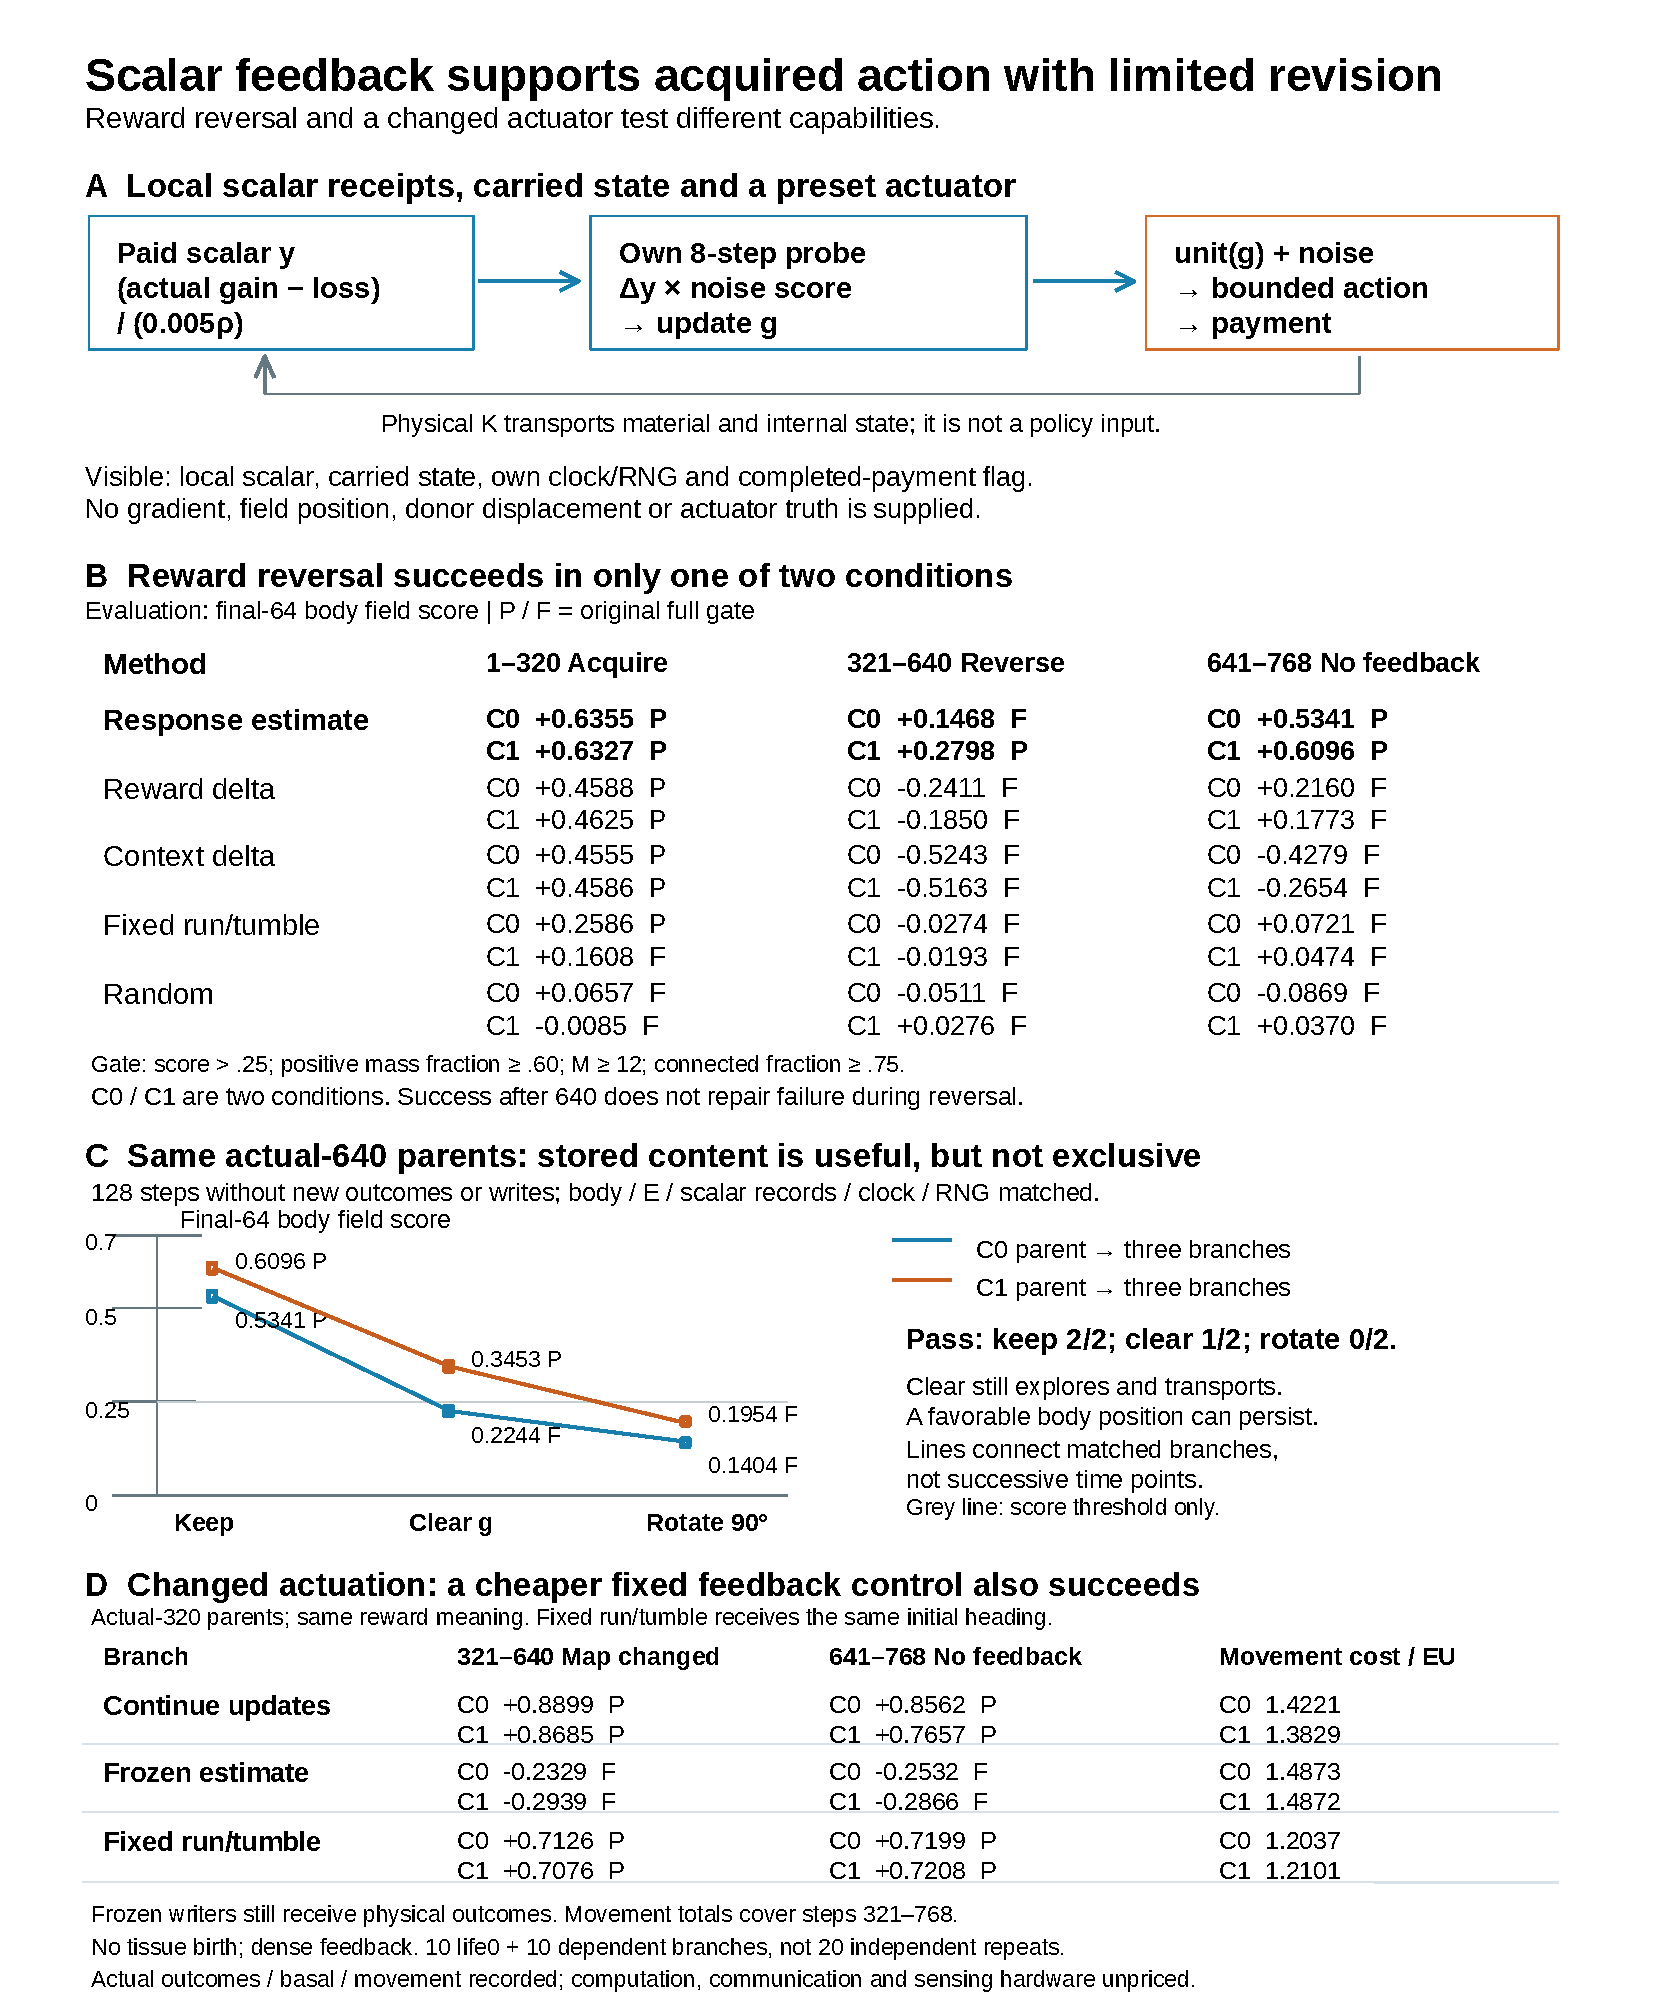
\includegraphics[width=\linewidth,height=0.68\textheight,keepaspectratio]{work/longform_v047/figures/scalar_action_v048/scalar_action.pdf}
\captionsetup{font=footnotesize}
\caption{\textbf{Scalar-only experience supports action acquisition, with different limits under reward and execution changes.}
\textbf{a}, A standard local response estimate uses completed scalar outcome changes and physically carried perturbation records. The transport operator $K$ moves material and internal state but provides no learner-facing displacement, gradient, field coordinate or actuator truth. Motion axes, cohesion, exploration and energy measurement are supplied.
\textbf{b}, All five methods, two paired seed--actuator conditions and three phases. Cells give final-64 mass-weighted field scores and the original complete gate (P/F); these evaluation quantities are not policy inputs. Response estimation passes acquisition in both conditions, reward reversal in one and the following no-new-feedback interval in both. The later success does not revise the failed reversal.
\textbf{c}, Two actual step-640 parents with response retained, cleared or rotated. Lines join related content interventions, not successive times. Retention passes twice, clearing once and rotation never. Clear branches still explore and move; rotation preserves response norm but not each bounded command or expense. Retained tails reuse recorded trajectories without replay.
\textbf{d}, From actual step-320 parents, only the physical execution map changes. Continued estimation and fixed run/tumble both pass the paid and later no-new-feedback windows in both conditions; frozen estimation fails. The fixed control receives the same acquired initial heading and spends less on movement. Expenditure sums both continuation phases. Ten new life-zero paths and ten dependent branches are not twenty independent repetitions. The conservative host has no tissue birth; physical expense is reported without a separate tariff for computation or sensing hardware. All phase outcomes and accounts are retained in the accompanying scalar-action source tables.}
\label{fig:scalar-action}
\end{figure}

